\documentclass[12pt]{report}
\usepackage{polyglossia} % enable TeX to generate text in target language. Also add support to languages (correct quoting style, etc.)
\setmainlanguage{french}
\usepackage{csquotes} % required to use polyglossia apparently, also handle quotes
\usepackage{fancyvrb} % insert content without interpreting as LaTeX
\usepackage[backend=biber]{biblatex} % bibliography management
\addbibresource{references.bib}
\usepackage[pdfborder={0 0 0.6}]{hyperref} % add hypertext reference support to navigate from and within the document
\usepackage{float} % to correctly position images or any figure environment
\usepackage{graphicx} % manage images
\graphicspath{ {./images/} } % set default path to images
\usepackage{wrapfig}
\restylefloat{figure} % again, to correctly position images or any figure environment
\usepackage{hyperref} % manage URL
\usepackage{appendix} % manage annexe numbering
\usepackage{pdfpages} % to insert pdf
\usepackage{listings} % to insert programming source code
\usepackage{color} % color for programming source code
\usepackage[acronym,toc]{glossaries} % to make a glossary

\loadglsentries{acronyms.tex}
\loadglsentries{glossaries.tex}
\makeglossaries

\lstset
{ %Formatting for code in appendix
    basicstyle=\footnotesize,
    numbers=left,
    stepnumber=1,
    showstringspaces=false,
    tabsize=1,
    breaklines=true,
    breakatwhitespace=false,
    numberstyle=\tiny\color{gray},
    keywordstyle=\color{blue},
    stringstyle=\color{red},
    commentstyle=\color{gray}
}

% custom handling of footnotes so I don't have to put them inline or manager counting myself
\newcounter{footnoteMarkCount}
\newcounter{footnoteTextCount}
\newcommand{\fnmark}{\stepcounter{footnoteMarkCount}\setcounter{footnote}{\value{footnoteMarkCount}}\addtocounter{footnote}{-1}\footnotemark}
\newcommand{\fntext}[1]{\stepcounter{footnoteTextCount}\setcounter{footnote}{\value{footnoteTextCount}}\footnotetext{#1}}

\begin{document}
    %%%%%%%%%%%%%%%%%%%%%%%%%%%%%%%%%%%%%%%%%
% University Assignment Title Page
% LaTeX Template
% Version 1.0 (27/12/12)
%
% This template has been downloaded from:
% http://www.LaTeXTemplates.com
%
% Original author:
% WikiBooks (http://en.wikibooks.org/wiki/LaTeX/Title_Creation)
%
% License:
% CC BY-NC-SA 3.0 (http://creativecommons.org/licenses/by-nc-sa/3.0/)
%
% Instructions for using this template:
% This title page is capable of being compiled as is. This is not useful for
% including it in another document. To do this, you have two options:
%
% 1) Copy/paste everything between \begin{document} and \end{document}
% starting at \begin{titlepage} and paste this into another LaTeX file where you
% want your title page.
% OR
% 2) Remove everything outside the \begin{titlepage} and \end{titlepage} and
% move this file to the same directory as the LaTeX file you wish to add it to.
% Then add \input{./title_page_1.tex} to your LaTeX file where you want your
% title page.
%
%%%%%%%%%%%%%%%%%%%%%%%%%%%%%%%%%%%%%%%%%
\begin{titlepage}

    \pagenumbering{gobble} % titlepage is not numbered

    \newcommand{\HRule}{\rule{\linewidth}{0.5mm}} % commmand to make horizontal lines

    \center

    %----------------------------------------------------------------------------------------
    %	HEADING SECTIONS
    %----------------------------------------------------------------------------------------

    \textsc{\LARGE IFOSUP}\\[0.5cm]
    \textsc{\large Institut de Formation Supérieure de la Ville de Wavre}\\[1.5cm]
    \textsc{\Large Bachelier en informatique de gestion}\\[0.5cm]
    \textsc{\large Épreuve intégrée}\\[0.5cm]

    %----------------------------------------------------------------------------------------
    %	TITLE SECTION
    %----------------------------------------------------------------------------------------

    \HRule \\[0.4cm]
    { \huge \bfseries Click and Run}\\[0.4cm]
    \textsc{\large Une application web modulaire pour automatiser les tâches récurrentes}\\[0.5cm]
    \HRule \\[1.5cm]

    %----------------------------------------------------------------------------------------
    %	AUTHOR SECTION
    %----------------------------------------------------------------------------------------

    \begin{minipage}{0.4\textwidth}
        \begin{flushleft} \large
        \emph{Auteur:}\\
        Adrien \textsc{Horgnies}
        \end{flushleft}
    \end{minipage}
    ~
    \begin{minipage}{0.4\textwidth}
        \begin{flushright} \large
        \emph{Directeur de projet:} \\
        Grégory \textsc{Schiano}
        \end{flushright}
    \end{minipage}\\[2cm]

    %----------------------------------------------------------------------------------------
    %	DATE SECTION
    %----------------------------------------------------------------------------------------

    {\large 2018~-~2019}\\[2cm]

    %----------------------------------------------------------------------------------------

    \vfill

\end{titlepage}
 % title page occupies first page
    \clearpage
\newpage
\pagenumbering{gobble}
\null
\clearpage
 % title page must be followed by an ampty page
    %%%%%%%%%%%%%%%%%%%%%%%%%%%%%%%%%%%%%%%%%
% University Assignment Title Page
% LaTeX Template
% Version 1.0 (27/12/12)
%
% This template has been downloaded from:
% http://www.LaTeXTemplates.com
%
% Original author:
% WikiBooks (http://en.wikibooks.org/wiki/LaTeX/Title_Creation)
%
% License:
% CC BY-NC-SA 3.0 (http://creativecommons.org/licenses/by-nc-sa/3.0/)
%
% Instructions for using this template:
% This title page is capable of being compiled as is. This is not useful for
% including it in another document. To do this, you have two options:
%
% 1) Copy/paste everything between \begin{document} and \end{document}
% starting at \begin{titlepage} and paste this into another LaTeX file where you
% want your title page.
% OR
% 2) Remove everything outside the \begin{titlepage} and \end{titlepage} and
% move this file to the same directory as the LaTeX file you wish to add it to.
% Then add \input{./title_page_1.tex} to your LaTeX file where you want your
% title page.
%
%%%%%%%%%%%%%%%%%%%%%%%%%%%%%%%%%%%%%%%%%
\begin{titlepage}

    \pagenumbering{gobble} % titlepage is not numbered

    \newcommand{\HRule}{\rule{\linewidth}{0.5mm}} % commmand to make horizontal lines

    \center

    %----------------------------------------------------------------------------------------
    %	HEADING SECTIONS
    %----------------------------------------------------------------------------------------

    \textsc{\LARGE IFOSUP}\\[0.5cm]
    \textsc{\large Institut de Formation Supérieure de la Ville de Wavre}\\[1.5cm]
    \textsc{\Large Bachelier en informatique de gestion}\\[0.5cm]
    \textsc{\large Épreuve intégrée}\\[0.5cm]

    %----------------------------------------------------------------------------------------
    %	TITLE SECTION
    %----------------------------------------------------------------------------------------

    \HRule \\[0.4cm]
    { \huge \bfseries Click and Run}\\[0.4cm]
    \textsc{\large Une application web modulaire pour automatiser les tâches récurrentes}\\[0.5cm]
    \HRule \\[1.5cm]

    %----------------------------------------------------------------------------------------
    %	AUTHOR SECTION
    %----------------------------------------------------------------------------------------

    \begin{minipage}{0.4\textwidth}
        \begin{flushleft} \large
        \emph{Auteur:}\\
        Adrien \textsc{Horgnies}
        \end{flushleft}
    \end{minipage}
    ~
    \begin{minipage}{0.4\textwidth}
        \begin{flushright} \large
        \emph{Directeur de projet:} \\
        Grégory \textsc{Schiano}
        \end{flushright}
    \end{minipage}\\[2cm]

    %----------------------------------------------------------------------------------------
    %	DATE SECTION
    %----------------------------------------------------------------------------------------

    {\large 2018~-~2019}\\[2cm]

    %----------------------------------------------------------------------------------------

    \vfill

\end{titlepage}
 % and then a copy of itself (weird, I know)

	% set my own counter so that I can style it however I want
	\setcounter{page}{1}

	\chapter*{Licence}
	\VerbatimInput{LICENSE.txt}
	\clearpage

	% style page number with roman numbers
	\renewcommand{\thepage}{\roman{page}}

	\tableofcontents
	\clearpage

	% style page number with arabic numbers
	\renewcommand{\thepage}{\arabic{page}}
	
	\printglossary[type=\acronymtype,title=Acronymes]
	\printglossary[title=Glossaire]

	\chapter{Introduction}
\label{ch:introduction}

\paragraph{}
Ces quatre dernières années, j'ai suivi les études pour acquérir le bachelier en informatique de gestion.
Le développement informatique me donne l'impression que tout peut être automatisé.
Ce présent travail est un argument en faveur de cette assertion et un formidable défi aux compétences et connaissances acquises lors de ma formation.

\paragraph{}
Je travaille à Altissia depuis deux ans.
Je développe de nouvelles fonctionnalités, corrige des bogues et réalise différentes tâches opérationnelles.

\paragraph{}
Chez Altissia, ainsi que dans de nombreuses entreprises, je l'imagine, un tas de données sont manipulées.
Ces données peuvent être des données des clients, des données des utilisateurs, des données métiers, etc.
Et pour de nombreux employés, la méthode la plus simple de stocker ces données est le tableur et bien souvent, le tableur Excel.

Malheureusement, il arrive fréquemment que ces données soient mal formatées ou invalides et ne permettent pas leur exploitation par les logiciels cibles.
Il incombe alors au service informatique de régler ces soucis, car ils ont de meilleures connaissances du format requis et disposent des meilleurs outils pour les corriger.

\paragraph{}
À l'heure actuelle, nous utilisons un programme appelé \textit{Altissia-launcher}.
Ce programme valide les données contenues dans des classeurs Excel, il les manipule et les transforme afin qu'elles puissent être exploitées par d'autres logiciels de l'entreprise.

Malheureusement, cet outil est très loin d'être parfait.
Il n'est utilisable que par un développeur, car il ne dispose pas d'interface graphique; on l'exécute directement depuis l'\gls{a-edi}.
De plus, même pour le développeur, il est difficile d'utilisation, car pour mener à bien un processus complet, il reste nécessaire d'appliquer manuellement certaines tâches.
Il faut par exemple, déplacer ou copier des fichiers d'un endroit à l'autre, lancer plusieurs scripts dans un certain ordre, etc.
En fait, il est impératif de suivre une documentation\fnmark pas à pas sous peine de se tromper et de devoir recommencer.
Enfin, il utilise des technologies désuètes qui le rendent très difficile à maintenir ou à faire évoluer.

% \fntext{\textit{Integrated Development Environment} que l'on traduit environnement de développement intégré, est le logiciel qui permet d'écrire, tester et exécuter du code.}
\fntext{Vous pouvez trouver la documentation d'un de ces processus en annexe \ref{ch:altissia-launcher-doc}.}

\paragraph{}
Grégory, le directeur technique d'Altissia, m'a proposé de développer un nouvel outil qui aura pour but de supplanter \textit{Altissia-launcher}.

\paragraph{}
L'objectif de ce nouveau logiciel en plus de reprendre les fonctionnalités de son prédécesseur sera de proposer une interface graphique ergonomique afin qu'il puisse être utilisé par un acteur métier plutôt que par un développeur.
En fait, plutôt que d'être une solution concrète, cela sera un cadre de travail proposant aux développeurs les outils pour pouvoir implémenter tous les cas possibles et imaginables.


    \chapter{Contexte}
\label{ch:context}

\paragraph{}
Altissia développe des sites web pour apprendre les langues en ligne.
Ces sites web utilisent de très nombreuses sortes de données:
\begin{enumerate}
    \item Questions de test de niveau
    \item Leçons
    \item Activités
    \item Vidéos
    \item Images
    \item Sons
    \item Articles de presse
    \item Quiz
    \item Dictées
    \item Autres
\end{enumerate}
Ces données sont loin d'être figées, elles évoluent pour s'adapter aux intérêts des apprenants, aux évolutions des langues, pour apporter des corrections ou plus généralement pour améliorer l'expérience de l'utilisateur.

Dans un monde idéal, toutes ces données seraient manipulées par les acteurs métiers au travers d'outils dédiés qui modifieraient directement les données dans leur contexte d'exploitation.
Toutefois, afin de satisfaire les exigences et désidératas de nos clients dans les temps impartis, la conception du contenu supplante le développement de son outil d'édition.

\paragraph{}
Toutes ces données prennent presque toujours un format différent entre le moment où elles sont travaillées et le moment où elles sont disponibles sur une plateforme.
Par exemple, une question d'un test de niveau est représentée par une ligne d'un fichier Excel pour les linguistes qui les éditent, mais correspond à plusieurs entrées dans une base de données Elasticsearch pour l'application.

\paragraph{}
Il est donc impératif d'effectuer la conversion entre ces différents formats afin de nourrir les applications.


\paragraph{}
Altissia développe des sites web pour apprendre les langues en ligne.
Ces sites web utilisent de très nombreuses sortes de données:
\begin{enumerate}
    \item Questions de test de niveau
    \item Leçons
    \item Activités
    \item Vidéos
    \item Images
    \item Sons
    \item Articles de presse
    \item Quiz
    \item Dictées
    \item Autres
\end{enumerate}
Ces données sont loin d'être figées, elles évoluent pour s'adapter aux intérêts des apprenants, aux évolutions des langues, pour apporter des corrections ou plus généralement pour améliorer l'expérience de l'utilisateur.

Dans un monde idéal, toutes ces données seraient manipulées par les acteurs métiers au travers d'outils dédiés qui modifieraient directement les données dans leur contexte d'exploitation.
Toutefois, afin de satisfaire les exigences et désidératas de nos clients dans les temps impartis, la conception du contenu supplante le développement de son outil d'édition.

\paragraph{}
Toutes ces données prennent presque toujours un format différent entre le moment où elles sont travaillées et le moment où elles sont disponibles sur une plateforme.
Par exemple, une question d'un test de niveau est représentée par une ligne d'un fichier Excel pour les linguistes qui les éditent, mais correspond à plusieurs entrées dans une base de données Elasticsearch pour l'application.

\paragraph{}
Il est donc impératif d'effectuer la conversion entre ces différents formats afin de nourrir les applications.


\section{La demande initiale}
\label{sec:initial-request}

\paragraph{}
Nos plateformes utilisent toutes sortes de contenus.
Bien souvent, ces contenus utilisent en tout ou en partie du texte.
Ces données textuelles doivent respecter des formats bien spécifiques afin d'être compatibles avec nos plateformes.

Il aurait été idéal de créer des éditeurs spécialement conçus pour nos applications.
Toutefois, afin de satisfaire nos clients dans les temps impartis par les contrats, nous avons dû faire le choix d'utiliser des outils d'édition générique et dans la plupart des cas, nous utilisons Excel.

Excel ne permet pas d'implémenter toutes les règles que nos données doivent respecter.
En effet, certaines de nos règles métiers imposent de consulter nos bases de données \gls{g-mysql} ou encore nos \gls{a-api}.
Il est donc nécessaire d'implémenter l'authentification imposée par nos serveurs avec du code.

Microsoft a conçu le langage de programmation \gls{a-vba} pour étendre les capacités d'Excel\cite{o365devx_pris_nodate}.
Nous avons rapidement écarté cette option, car aucun de \textbf{nos développeurs} ne maitrise ce langage et il n'apporte que peu d'avantages comparés à d'autres langages que nous maitrisons déjà.

\paragraph{}
Altissia launcher est un projet Apache Ant\fnmark{} et constitue dans notre cas une bibliothèque de scripts.
Son principal rôle est la validation, la manipulation et l'import de données stockées dans des fichiers Excel.
Nous avons aussi implémenté des tâches similaires avec des scripts codés en Python\fnmark{} ou en \gls{g-java} avec le \gls{g-framework} \Gls{g-spring} Batch\fnmark{}.

\fntext{Apache Ant est un outil permettant de construire une application \gls{g-java} à partir de son code source. Une alternative plus connue est \href{https://maven.apache.org/}{Apache Maven}.}
\fntext{Python est un langage de programmation très populaire pour créer des scripts.}
\fntext{\Gls{g-spring} Batch est un composant du \textit{Framework} Spring permettant un traitement par lots de grandes quantités de données.}

\paragraph{}
Ces différents outils n'ont pas d'\textbf{interface graphique} propre et nous n'en avons développé aucune.
Pour le moment, lorsqu'un acteur métier a besoin d'un de ces scripts, il doit demander l'aide d'un développeur.

\paragraph{}
Les fichiers Excel sont stockés sur un \gls{a-nas} et travaillés par de multiples personnes.
Les règles qui régissent ces fichiers peuvent changer lorsque l'on se rend compte qu'elles permettent l'insertion de données inutilisables par les applications qui vont les consommer ou tout simplement lorsque notre contenu de cours évolue.
Il est donc important que chacun valide son travail avec la \textbf{dernière version} des règles de validation.

\paragraph{}
La demande initiale est de centraliser la validation de ces données dans une application web.

Cette application web devra utiliser les mêmes technologies que les autres sites utilisés par l'entreprise. À savoir que les sites web développés par Altissia utilisent le socle d'application Spring Boot pour la partie serveur et le \textit{framework} Angular pour la partie client\fnmark{}.

\fntext{Souvent, les sites web sont organisés en deux parties: la partie cliente que l'on télécharge en se rendant sur le site, elle affiche les pages web et la partie serveur qui nous transmet les données que l'on insère dans les pages.}


\section{Les produits existants}
\label{sec:existing-products}

\paragraph{}
Pour valider le contenu d'un fichier Excel, le premier outil auquel on a pensé est... Excel lui-même.
La raison pour laquelle on a écarté cette solution est que les règles que nous voulons implémenter sont spécifiques à nos besoins.
Il n'existe aucun produit qui implémente nos besoins.
Le mieux que nous pouvons trouver est un logiciel qui nous aide à créer notre solution.

Un logiciel tel qu’Excel impose le langage de programmation (VBA) et ne permet pas de réutiliser la base de code existante.

\paragraph{}
De plus, pour effectuer son travail, ce nouveau logiciel aura besoin de communiquer avec nos API.

\paragraph{}
Enfin, des librairies existantes fournissent toutes les fonctionnalités que l'on pourrait attendre d'une solution existante.

\paragraph{}
Nous sommes donc arrivés à la conclusion que la meilleure solution est de développer un nouveau logiciel.
Cela permettra d'avoir une solution flexible et parfaitement intégrée dans l'infrastructure existante.



	\chapter{Cahier des charges}
\label{ch:specifications}

\paragraph{}
L'application doit répondre aux besoins de la société Altissia.
Afin de m'accorder sur la manière dont l'application va y répondre, j'ai élaboré ce présent cahier des charges en collaboration avec de multiples employés d'Altissia.

\paragraph{}
Grégory Schiano est le directeur technique d'Altissia.
C'est avec lui que je vois comment intégrer ce nouveau logiciel au sein de l'architecture existante.

\paragraph{}
Renaud Laloux est un développeur expérimenté, il me conseille sur les choix techniques cruciaux.
Sa connaissance de la base de code et ses compétences me permettent d'éviter de nombreux pièges.

\paragraph{}
Sophie Roekhaut est une cheffe de projet qui est notamment responsable des contenus de cours.
Elle détermine le besoin, le présente sous forme de fonctionnalités et les ordonne par priorité.
Elle valide la complétion des fonctionnalités au fur et à mesure que je les lui soumets.

\paragraph{}
L'équipe des linguistes sera la première à bénéficier de ce nouvel outil.
Elles donnent leurs commentaires sur le travail fourni, expriment leur contentement et fournissent des pistes d'améliorations le cas échéant.


\section{Élaboration}
\label{sec:elaboration}

L'élaboration de ce cahier des charges s'est faite en deux phases. 
Dans un premier temps, j'ai participé à des réunions avec Grégory, Renaud et Sophie afin de démarrer le projet. 
Et dans un second temps, nous avons ajouté et adapté des fonctionnalités au fur et à mesure que le projet a avancé.

\paragraph{}
Altissia travaille selon les principes \Gls{g-agile} et plus précisément la méthodologie \Gls{g-scrum}.
Ces principes sont nés d'un constat sur les projets informatiques, la majorité échoue\cite{standish_standish_nodate} et la plupart du temps c'est parce que les besoins sont mal définis ou parce que la communication entre les parties prenantes est mauvaise (voir figure \ref{fig:why-projects-fails}).

\begin{figure}[ht]
    \centering
    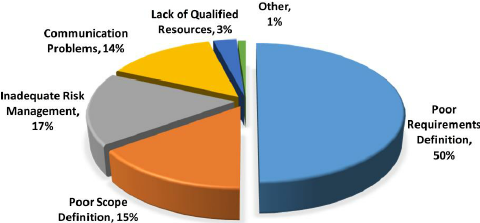
\includegraphics[scale=.8]{images/why-projects-fail.png}
    \caption{Role of Requirements in Software Project Failures. Source: ESI International Survey of 2000 Business Professionals, 2005.}
    \label{fig:why-projects-fails}
\end{figure}

\paragraph{}
Pour répondre à ces enjeux, le service informatique d'Altissia a adopté la méthode \Gls{g-scrum}.
Cela consiste à travailler de manière itérative, de régulièrement produire des résultats intermédiaires utilisables, d'impliquer les différents acteurs, d'obtenir leurs commentaires et d'adapter la direction du projet selon ceux-ci.

\paragraph{}
C'est donc pour cela que le cahier des charges n'est pas complet et définitif au début du projet, mais qu'il s'étoffe au fur et à mesure.


\subsection{Les interviews}
\label{subsec:interviews}

\paragraph{}
J'ai eu une première interview avec Grégory pour définir le besoin général et le contexte qui l'entoure.
Il explique qu'en facilitant la vérification et la conversion des nouveaux contenus des cours, l'application permettrait d'accélérer l'intégration des nouveaux contenus de cours dans nos plateformes.

Nous discutons de la forme que cette application va prendre. 
Je propose de la structurer en trois parties: une librairie applicative, un serveur et une libraire de composants web.
Après discussions, nous concluons qu'il n'est pas utile de former une librairie et que de directement intégrer les fonctionnalités dans un serveur simplifiera le développement.

Il s'agit donc de créer une application serveur qui s'occupe de la manipulation des données et une application cliente qui affiche les données et enregistre les choix de l'utilisateur.
Sous cette forme, Altissia pourra facilement personnaliser\fnmark{} l'application pour l'intégrer aux logiciels existants.
\fntext{Il s'agit ici de faire un \textit{fork} de l'application. Une sorte de copie que l'on personnalise sans modifier l'originale, mais qui peut toujours obtenir les dernières mises à jour de la source.}

\paragraph{}
Ensuite, j'ai eu une réunion avec Renaud et Sophie.
À deux, ils ont défini précisément les problèmes de l'outil existant et pourquoi on veut le remplacer.

Renaud connait très bien l'outil que l'on veut remplacer, Altissia launcher, il m'a expliqué les difficultés rencontrées pendant son développement et comment il a terminé dans son état actuel.
La principale cause est le temps de développement nécessaire pour prendre en charge de nouveaux formats et la difficulté d'utilisation qui encourage les utilisateurs à s'en passer.

Sophie a établi la liste des manquements du logiciel actuel qu'il faudrait suppléer et les fonctionnalités qu'elle voudrait ajouter.
Certaines règles ne sont pas vérifiées, les codes d'erreur sont cryptiques et certaines informations pourraient accompagner les erreurs afin d'en faciliter la correction.

\paragraph{}
Par la suite, nous avons continué de nous rencontrer dans le cadre des réunions SCRUM:
\begin{itemize}
    \item Le \textit{daily standup}: courte réunion quotidienne pour informer de l'avancement et toute difficulté rencontrée
    \item Le \textit{sprint planning}: Réunion bimensuelle où l'on planifie les deux prochaines semaines
    \item Le \textit{backlog refinement}: Réunion bimensuelle où l'on clarifie la définition des fonctionnalités pour s'assurer qu'elles sont correctement comprises et prêtes à être implémentées.
    \item La \textit{Review}: Réunion bimensuelle en fin de sprint où l'on présente les résultats produits durant la période à toutes personnes intéressées.
\end{itemize}

    
\subsection{Les demandes clients}
\label{subsec:customer-requests}

Voici les différentes fonctionnalités établies au cours de l'élaboration du cahier des charges:
\begin{enumerate}
    \item Valider de fichiers Excel:
    \begin{enumerate}
        \item Présence des feuilles
        \item Présence des entêtes
        \item Ignorer les entêtes superflus
        \item Le respect d'un modèle de chaine de caractères (une \gls{g-regex}).
        \item La position d'une valeur numérique par rapport à une borne inférieure
        \item La position d'une valeur numérique par rapport à une borne supérieure
        \item L'inclusion d'une valeur numérique entre deux bornes
        \item Le résultat de l'évaluation d'une \gls{g-bool-func} arbitraire
        \item La taille d'une chaine de caractères
        \item L'appartenance d'une valeur à un ensemble fini
        \item La contrainte de référence\fnmark{} entre deux feuilles du même classeur
        \item La contrainte de référence dans une base de données
        \item La contrainte de référence dans un API externe
        \item L'unicité d'une valeur au sein de sa colonne
        \item L'unicité d'une combinaison de valeurs au sein de sa feuille
        \item Validation d'une cellule en fonction de la valeur d'une autre cellule
        \item Le \gls{g-null}
        \item Le respect du format des \textit{mails}
    \end{enumerate}
    \item Contrôler l'application depuis une interface web:
    \begin{enumerate}
        \item Soumettre un fichier pour validation
        \item Visualiser la validation
        \item Soumettre un fichier pour exécution
        \item Visualiser le résultat de l'exécution
        \item Visualiser l'historique des exécutions
        \item Être notifié de la complétion d'une validation ou exécution
    \end{enumerate}
\end{enumerate}
    
\fntext{Une contrainte de référence signifie qu'une valeur doit exister dans le référentiel. Par exemple, mon nom de famille doit être porté par l'un de mes parents pour que je puisse le porter.}
% \fntext{En informatique, la nullité indique l'absence de valeur.}


\subsection{Les propositions au client}
\label{subsec:proposals-to-customer}

\paragraph{}
Le logiciel élaboré est le résultat d'un dialogue constant entre le développeur et les acteurs métiers.

Toutes les fonctionnalités implémentées sont issues de propositions de ma part afin de satisfaire les besoins qui me sont soumis.

\paragraph{}
Toutefois, certaines fonctionnalités ont trouvé leur origine dans des propositions spontanées plutôt que dans des discussions.

\paragraph{}
Une première proposition a été de séparer la phase de traitement et la phase de validation.
En effet, seule la phase de traitement existait. 
Lorsque l'on tentait de soumettre un fichier, soit cela réussissait, soit cela échouait et l'on recevait les journaux de l'application\fnmark.
\fntext{Les journaux d'application sont des messages écrits par des développeurs à l'intention d'autres développeurs.}
% TODO diagramme d'activité

Une première phase de validation permet de récupérer un rapport de validation.
Une seconde phase, répète la première pour s'assurer de la validité des données, renvoie une erreur en cas d'échec\fnmark, traite les données en cas de réussite et avertit l'utilisateur du succès.
\fntext{Ce n'est pas censé arriver! Le traitement doit être accessible uniquement après le succès de la première phase.}

Ce découpage permet à l'utilisateur de valider son travail au fur et à mesure plutôt que de le soumettre lorsqu'il est complet.
Cela permet de réduire la latence sur le retour d'information et d'encourager les utilisateurs à utiliser l'application.
% TODO diagramme d'activité

\paragraph{}
Un second exemple est le flux d'utilisation où j'ai proposé de réduire au maximum le nombre d'opérations.
Pour ce faire, j'ai créé une expérience linéaire où l'action suivante est la seule possible.

\begin{figure}[ht]
    \centering
    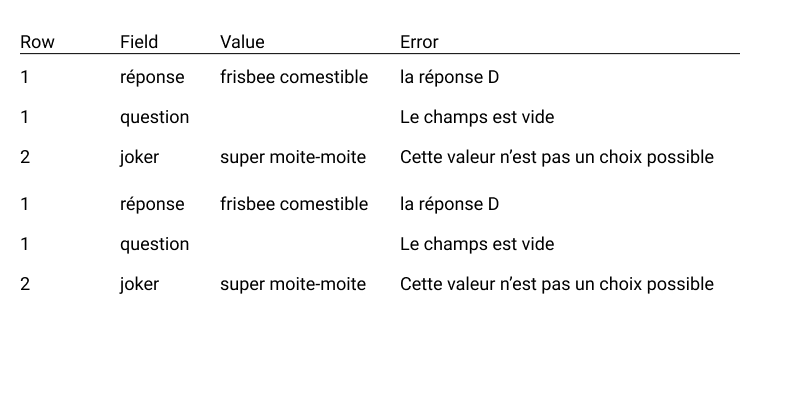
\includegraphics[width=0.7\textwidth]{images/prototypes/spreadsheet-validation.png}
    \caption{Le composant pour visualiser le rapport de validation}
    \label{fig:spreadsheet-validation}
\end{figure}
Ainsi, afin de valider un classeur, observer le succès ou l'échec de la validation, voir le rapport de validation (voir figure \ref{fig:spreadsheet-validation}), soumettre le classeur pour traitement et observer le succès de son traitement, seules deux actions sont requises:
\begin{enumerate}
    \item Glisser et déposer le fichier dans la zone prévue (voir figure \ref{fig:spreadsheet-handler}).
    \item Cliquer sur le bouton prévu pour le traitement.
\end{enumerate}
Cette simplification a pour but d'encourager l'utilisation fréquente de l'application.
\begin{figure}[ht]
    \centering
    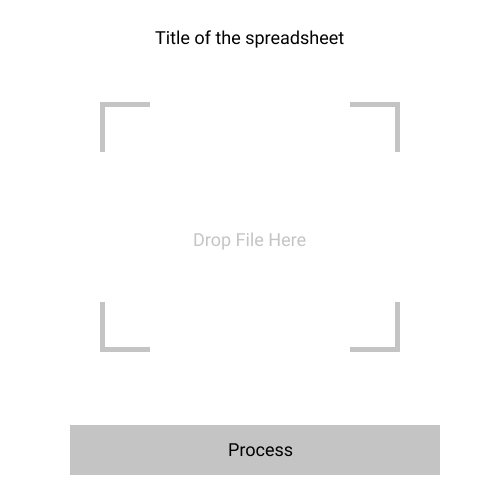
\includegraphics[width=0.7\textwidth]{images/prototypes/spreadsheet-handler.png}
    \caption{Le composant pour recevoir et soumettre les fichiers}
    \label{fig:spreadsheet-handler}
\end{figure}



\section{Lots d'informations identifiés}
\label{sec:identified-information-packages}
La nouvelle application est un outil qui transforme des données, mais n'utilise pas de données propres.

Altissia a fait le choix de structurer ses fonctionnalités en microservice.
Cela veut dire que chaque service a des responsabilités délimitées et que si un service a besoin de ressources qu'il n'a pas en interne, il appelle le service responsable.
Les données vont transiter par la nouvelle application pour rejoindre le service pertinent.

Par exemple, pour l'authentification, la nouvelle application s'adressera au service dédié et en cas de succès, recevra un \gls{a-jwt} qui lui permettra de communiquer avec les autres \gls{a-api}.
Ceci alors même que l'application n'a pas accès à la base de données des utilisateurs.



\section{Les acteurs de l'environnement d'exploitation de l'application}
\label{sec:application-prod-env-actors}

\paragraph{}
Les utilisateurs seront forcément des employés d'Altissia.
L'application est dans un premier temps conçue pour répondre aux besoins de l'équipe des \textbf{linguistes}.
Toutefois, un besoin existe aussi dans l'\textbf{équipe commerciale} et l'\textbf{équipe de communication} et ils auront le plaisir de les satisfaire avec ce nouvel outil dans un futur proche.

\paragraph{}
Par simplicité, l'ajout de nouvelles fonctionnalités se fera en déployant de nouvelles versions de l'application.
Pour pouvoir gérer de nouveaux documents, il sera donc nécessaire de faire appel aux développeurs.

Le déploiement en lui-même, le fait de rendre l'application disponible aux utilisateurs finaux est géré par l'équipe des \textbf{devops}\fnmark.

\fntext{\textit{Devops} est la contraction des termes \textit{developers} et \textit{operations} et qui identifient les personnes responsables du déploiement des applications. Ils mettent le travail des développeurs dans les mains des utilisateurs.}


\section{Définition de la première version de l'application}
\label{sec:first-version-definition}

Les besoins sont nombreux, mais il est nécessaire de s'arrêter sur un périmètre défini pour une première version.
Cela permettra d'obtenir un retour d'information sur les choix pris et de s'adapter aux besoins.

\subsection{Besoins métiers}
\label{subsec:business-needs}

\paragraph{}
La première version de l'application aura pour but de satisfaire un besoin dans le cadre de la prochaine version de l'application mobile de cours en ligne qui est déployé le 20 mai 2019.
Spécifiquement, les éléments de structure des cours ont été écrits dans plusieurs classeurs Excel.
Il faut valider leur format et utiliser les données pour créer les entrées correspondantes dans une base de données MySQL.
Ces éléments de structure sont les suivants:
\begin{itemize}
    \item Parcours d'apprentissage
    \item Mission
    \item Leçon
    \item Activité
    \item Exercice
\end{itemize}

Ces structures comportent toutes sortes d'attributs dont les valeurs doivent respecter leur domaine de définition.
Ces attributs sont par exemple: des titres, des identifiants, des niveaux de difficulté, des thèmes (job, vacances, vie quotidienne, etc.) ou encore des sujets d'apprentissages (prononciation, grammaire, etc.).

\paragraph{}
Par exemple, parmi les attributs, il y a le code de la langue qui doit être au format de la norme \textit{RFC 4647}\cite{davis_matching_nodate} (4 lettres séparées par un trait d'union ou un trait de soulignement).
Le niveau de difficulté est un élément de la liste du cadre européen commun de référence pour les langues\cite{noauthor_cadre_nodate}: A1, A2, B1, B2, C1 et C2.
Le type de la leçon est un mot parmi une liste finie.
Le titre de la leçon est une suite de mots arbitraires.
Le type de l'activité est un mot parmi une liste finie.
Le titre de l'activité est une suite de mots.

Chaque attribut apporte ses propres contraintes.

\paragraph{}
Il en résulte que pour la première version, il est nécessaire de pouvoir évaluer:
\begin{itemize}
    \item Le respect d'un modèle de chaine de caractères (une \gls{g-regex}).
    \item La position d'une valeur numérique par rapport à une borne inférieure
    \item La position d'une valeur numérique par rapport à une borne supérieure
    \item L'inclusion d'une valeur numérique entre deux bornes
    \item L'appartenance d'une valeur à un ensemble fini
    \item Le résultat de l'évaluation d'une fonction\fnmark booléenne arbitraire
    \fntext{Il est question ici d'une fonction informatique, en l'occurrence, elle transforme une valeur de son domaine de définition en une réponse vraie ou faux. Une même entrée donne toujours la même sortie.}
    \item La taille d'une chaine de caractères
    \item La contrainte de référence\fnmark dans une base de données
    \fntext{Une contrainte de référence signifie qu'une valeur doit exister dans le référentiel. Par exemple, mon nom de famille doit être porté par l'un de mes parents pour que je puisse le porter.}
    \item La contrainte de référence dans un API externe
    \item La contrainte de référence entre deux feuilles du même classeur
    \item La nullité\fnmark d'une valeur
    \fntext{En informatique, la nullité indique l'absence de valeur.}
    \item Le respect du format des \textit{mails}
    \item L'appartenance d'une valeur à un ensemble
    \item L'unicité d'une valeur au sein de sa colonne
    \item L'unicité d'une combinaison de valeurs au sein de sa feuille
\end{itemize}

\subsection{Besoins techniques}
\label{subsec:tech-needs}

\paragraph{}
Afin d'avoir une gestion centrale de l'application et de s'assurer que la dernière version est toujours utilisée, nous avons fait le choix d'implémenter la solution sous la forme d'un site web.
Ce choix était particulièrement évident, car c'est le coeur de métier d'Altissia et que l'entreprise dispose de très bonnes compétences en la matière.

\paragraph{}
Ce site web sera composé d'un serveur et d'une application cliente.
Le serveur s'occupe de la validation et du traitement des données.
L'application cliente présente les informations de manière visuelle et compréhensible et donne le contrôle à l'utilisateur.

\paragraph{}
Ce site web devra répondre aux impératifs de qualité et de sécurité d'Altissia.
Cela inclut l'utilisation du système d'authentification existant, l'utilisation du système de licences\fnmark pour gérer les droits des utilisateurs, système de surveillance de la santé du serveur ainsi que les outils d'administration habituels. % TODO maybe put some examples or ref to detailed list
\fntext{Un utilisateur peut avoir plusieurs licences. Chaque service peut exiger certaines licences pour certaines fonctionnalités. Par exemple, l'administration des utilisateurs requiert les droits d'administrateur.}
De plus, sur le plan technique, cela impose d'utiliser la même structure et les mêmes technologies que les applications existantes.
Ces technologies sont détaillées dans le chapitre \ref{ch:analysis}.


\section{Perspectives d'évolution pour une version ultérieure}
\label{sec:future-release-outlook}

Du fait qu’Altissia travaille selon le cadre de travail Agile, de nombreuses fonctionnalités sont imaginées et priorisées selon les besoins du moment, l'état actuel du développement et d'autres facteurs.
De nombreuses fonctionnalités sont donc envisageables, mais toutes ne quitteront pas le \textit{backlog}\fnmark
\fntext{Le backlog est le document qui regroupe toutes les fonctionnalités imaginées. Elles y restent tant qu'elles ne sont pas inscrites au planning.}

\subsection{Prochaines fonctionnalités}
\label{subsec:next-features}

Les prochaines fonctionnalités sont celles qui sont estimées les plus importantes et situées dans le haut de la pile.

Les fonctionnalités les plus attendues sont:
\begin{itemize}
    \item Détection du type de classeur: Plutôt que l'utilisateur choisisse le modèle de classeur qu'il veut utiliser, il dépose son classeur et le programme détecte à quel modèle il correspond.
    \item Téléchargement d'un modèle d'un classeur: L'utilisateur choisit un modèle de classeur et télécharge un fichier exemplaire.
    \item Traitement par lot: L'utilisateur peut soumettre de multiples fichiers en une seule passe.
    \item Gestion asynchrone: L'utilisateur lance une action et ne doit pas attendre la fin de celle-ci pour lancer l'action suivante.
    \item Notification: L'utilisateur est notifié lors de la fin d'une tâche.
\end{itemize}

\paragraph{}
Lorsqu'un utilisateur travaille avec plusieurs modèles de classeur, lui ôter la tâche de devoir choisir le bon modèle à chaque fois qu'il passe d'un fichier à un autre va lui permettre de gagner du temps.

\paragraph{}
Habituellement, l'utilisateur arrive sur l'application avec des fichiers existants. Toutefois, afin d'accommoder plus facilement les nouveaux utilisateurs, leur permettre d'obtenir des modèles sur l'application plutôt que dans les dossiers partagés ou en demandant à un collègue permettra de réduire les risques d'erreur et le travail de recherche.

\paragraph{}
Certains cas d'utilisation nécessitent de stocker les informations dans de multiples fichiers pour le même modèle.
C'est par exemple le cas pour certains modèles de classeur ou chaque fichier ne contient les données que pour une langue.
Il y a donc un classeur par langue.
Certaines linguistes travaillent parfois sur plusieurs langues en même temps.
La soumission multiple permettra un gain de temps.

\paragraph{}
La gestion asynchrone permettra de rendre le contrôle à l'utilisateur lors du traitement de fichiers volumineux ou dont les données sont lentes à traiter.
En effet, certains fichiers contiennent plusieurs dizaines de milliers de lignes.
D'autres fichiers sont lents à traiter à cause des nombreux appels aux réseaux.

\paragraph{}
Du fait de la gestion asynchrone, il est nécessaire de pouvoir notifier un utilisateur de la fin d'une tâche afin qu'il n'ait pas besoin de visiter fréquemment la page des résultats.

\subsection{Pré-requis techniques}
\label{subsec:nex-version-technical-requirements}

\paragraph{}
La détection du type de classeur, le téléchargement d'un modèle et le traitement par lot peuvent être ajoutés avec les technologies déjà intégrées.

Par contre, la gestion asynchrone et les notifications nécessitent l'introduction d'une nouvelle technologie.
L'outil qui remplit ce cas d'utilisation est appelé un agent de messages.
Altissia utilise déjà une telle technologie dans d'autres situations et je compte donc utiliser la même solution : \textit{RabbitMQ}.

\paragraph{}
Un agent de message est un logiciel qui stocke des messages dans des fils et les conserve jusqu'à ce qu'ils soient consommés.
Ainsi, le serveur enverra le résultat de son travail à l'agent de message plutôt que directement à l'utilisateur.
Ceci, car ce logiciel est capable de conserver le message et le délivrer quand l'utilisateur est prêt à le recevoir.



    \chapter{Analyse}
\label{ch:analysis}

Afin de structurer et formaliser les besoins des utilisateurs dans le but d'assurer la compréhension entre les différents partis, j'ai choisi de les représenter sous forme de diagrammes.
Je me suis notamment servi de la norme \gls{a-uml} sans pour étant m'y restreindre.
L'\gls{a-uml} est un standard d'industrie qui permet de représenter des informations de manière univoque.
Bien que ce soit sensé être un standard, les différentes implémentations disponibles sur le marché se distinguent les unes des autres et il peut être utile de noter que j'ai utilisé le logiciel \guillemotleft{} Visual Paradigm Modeler Edition \guillemotright{} en version 15.2.

Je ne me suis pas restreint à cette norme car tous les participants du projet ne la maitrisent pas.
Les clients du projet n'y sont pas formés et sont pourtant bien souvent les principaux intéressés.

\section{Les cas d'utilisation}
\label{sec:use-cases}

\paragraph{}
Le seul besoin métier est la validation de fichiers Excel contenant des données utiles à l'accomplissement du travail de l'utilisateur. Toutefois, la mise en place d'un site web implique la gestion d'autres aspects comme la sécurité ou l'administration du site web.

\paragraph{}
On distingue trois types d'utilisateurs qui n'ont pas accès aux mêmes fonctionnalités:
\begin{itemize}
    \item Le \textbf{visiteur}: Il n'a accès à rien si ce n'est l'accès à l'authentification afin de gagner les privilèges de l'\textbf{utilisateur}.
    \item L'\textbf{utilisateur}: Il a accès aux fonctionnalités qui font le coeur de l'application. Cette dernière est conçu pour lui.
    \item L'\textbf{administrateur}: Il a tous les droits de l'utilisateur normal avec en plus la possibilité d'accéder aux outils d'administration qui permettent notamment de modifier les paramètres du serveur ainsi que les utilisateurs eux-même.
\end{itemize}

A partir d'ici, je mettrai ces trois termes en gras lorsque je ferai explicitement référence aux définitions présentes ci-dessus plutôt qu'à celles de la langue française.

\subsection{La liste des cas d'utilisation}
\label{subsec:use-cases-list}

\begin{figure}[ht]
    \centering
    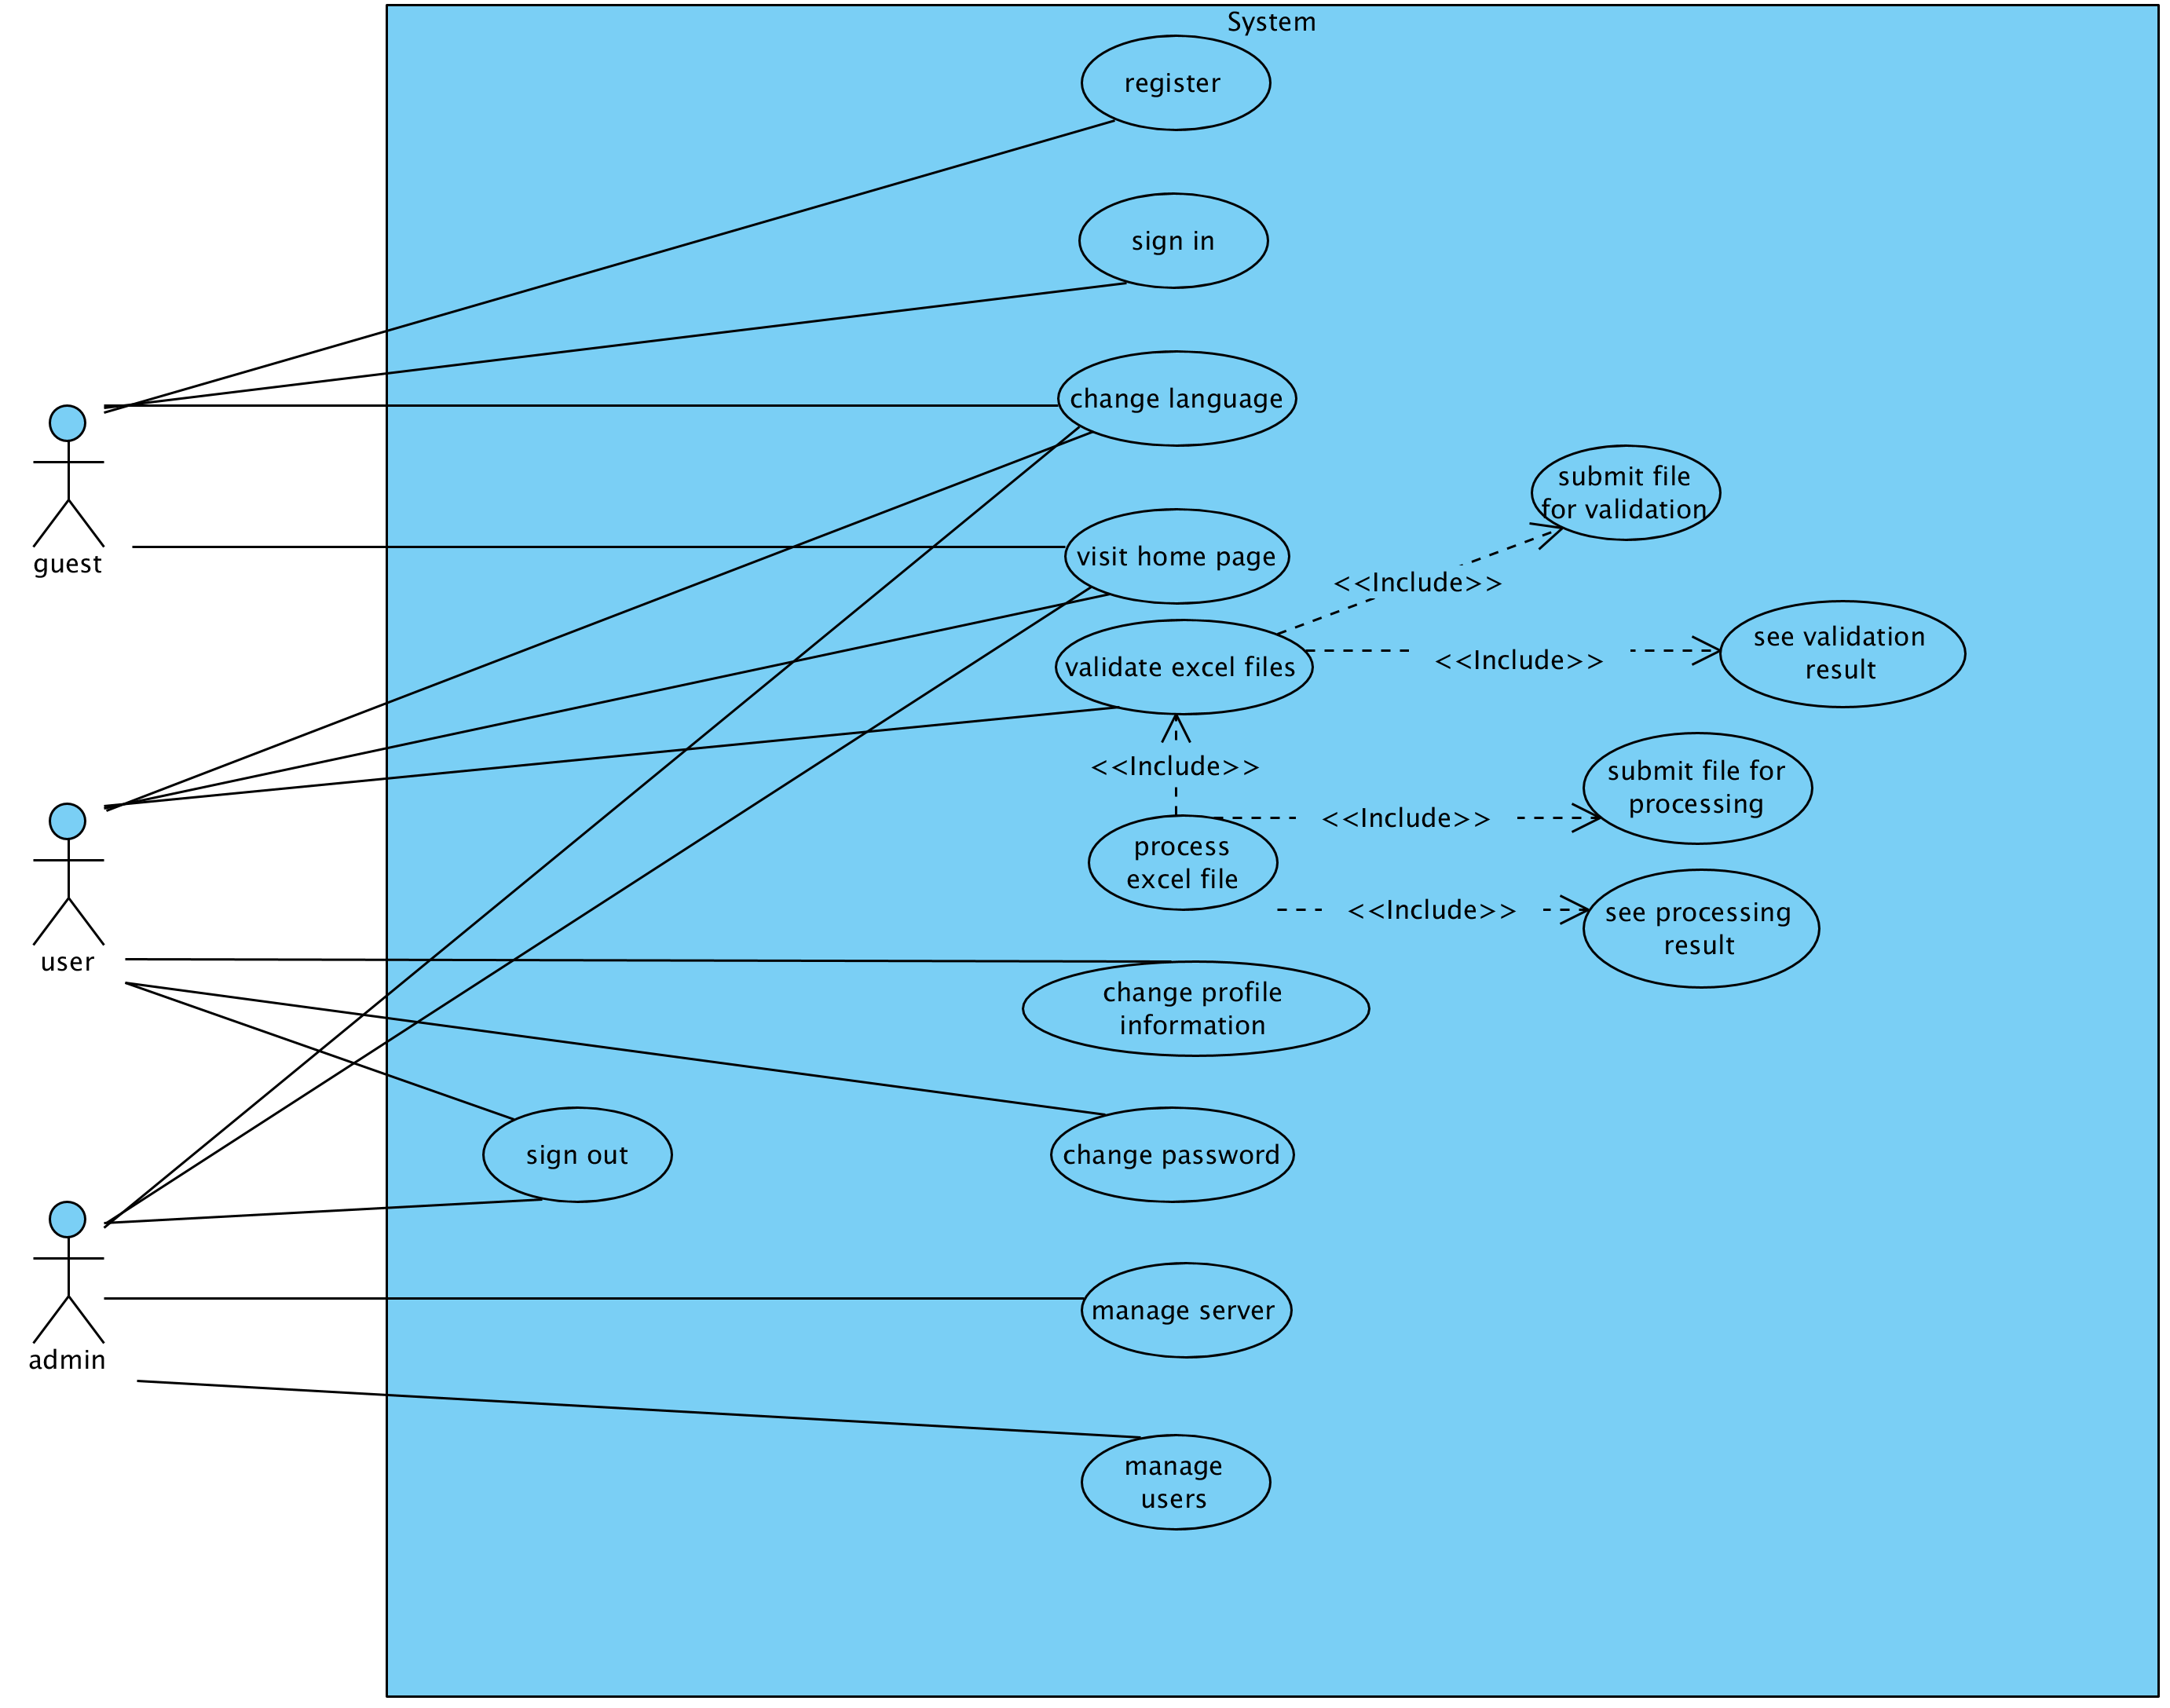
\includegraphics[width=0.8\textwidth]{images/diagrams/use-cases-macro.png}
    \caption{Les cas d'utilisation}
    \label{fig:use-cases-macro}
\end{figure}

\paragraph{}
Le diagramme \ref{fig:use-cases-macro} liste les différents cas d'utilisation et en l'analysant avec attention, on peut observer certains faits qui sont à première vue contre intuitifs.

\paragraph{}
Dans de nombreuses applications, on pourrait considérer une sorte d'héritage entre les différents niveaux de privilèges parmi les utilisateurs. Hors, ce n'est pas le cas ici. En effet, seul le \textbf{visiteur} a accès aux fonctionnalités pour s'enregistrer et se connecter. Plus surprenant, l'\textbf{administrateur} n'a pas accès aux fonctionnalités du coeur de l'application que sont la validation et le traitement des classeurs Excel. Encore plus étonnant, l'administrateur ne peut n'y accéder à son profil, n'y changer son mot de passe.

\begin{figure}[ht]
    \centering
    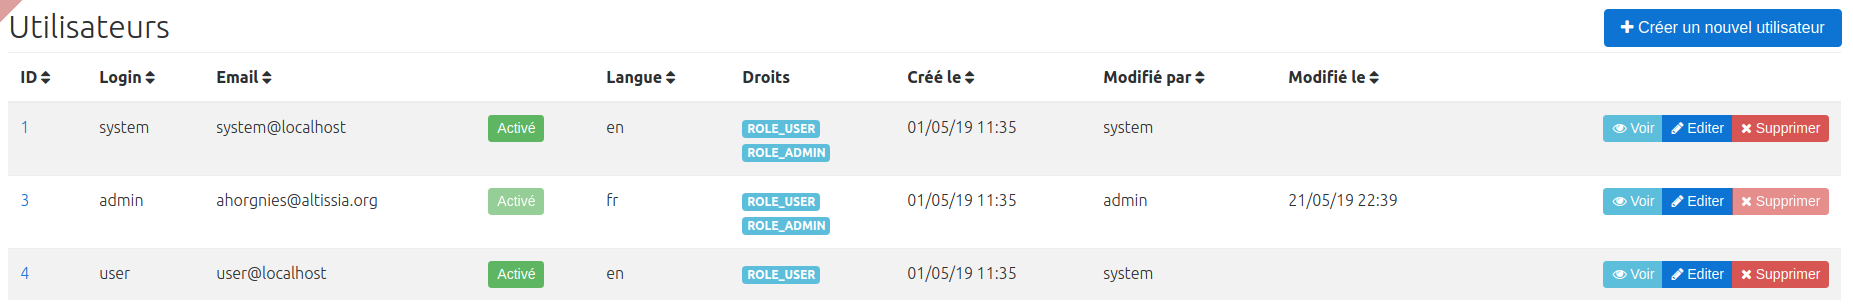
\includegraphics[width=0.8\textwidth]{images/screenshot/screenshot-user-admin-page.png}
    \caption{Une capture d'écran de la page de gestion des utilisateurs}
    \label{fig:user-admin-page}
\end{figure}

\paragraph{}
Cela est du au fait que les permissions sont gérées par un système de licences. Une personne peut cumuler les licences. Ainsi, plutôt que de faire hériter un rôle d'un autre, nous avons choisis de lier les permissions aux licences et de donner autant de licences que nécessaires aux personnes. Cela permet une gestion plus fine des autorisations et aussi plus simple à mettre en place.

Grâce à cela, la nouvelle application peut être déployé avec la base des utilisateurs existante complète sans risquer de compromettre les ressources qu'elle expose. En effet, seuls les personnes qui recevront la licence appropriée auront réellement accès à l'application.

De ce fait, un \textbf{visiteur} n'est pas une personne sans licence mais une personne qui n'a aucune licence adaptée.

Dans les faits, un \textbf{administrateur} aura toujours la licence d'un \textbf{utilisateur}. C'est ce que l'on peut observer sur l'image \ref{fig:user-admin-page}. Il a donc la double casque d'\textbf{administrateur} et d'\textbf{utilisateur}.

\paragraph{}
Le traitement inclue la validation. Bien que ces deux fonctionnalités soient fondamentalement distinctes, nous avons fait le choix d'inclure la validation comme première étape du traitement. Faire ainsi permet d'assurer la validité des données traitées et exclut toute erreur humaine.

\paragraph{}
Une chose qu'il n'est pas possible de voir sur ce diagramme \ref{fig:use-cases-macro} est que la validation et le traitement des classeurs sont des cas d'utilisation abstraits. En effet, il est nécessaire de les spécialiser sans quoi ils ne représentent rien.

Il faut se pencher sur des schémas plus détaillés pour comprendre ce que ces cas d'utilisation couvrent. C'est le sujet de la sous-section \ref{subsec:spreadsheet-use-case}.


\subsection{L'authentification}
\label{subsec:auth-feature}

\paragraph{}
L'authentification mise en place doit être compatible avec le système d'authentification présent sur les services d'Altissia. C'est particulièrement facile car c'est une authentification dite sans serveur. Cela veut dire qu'un client peut prouver son identité sans qu'un serveur tiers confirme les droits auxquels le \gls{g-client} prétend. 

\begin{figure}[h]
    \centering
    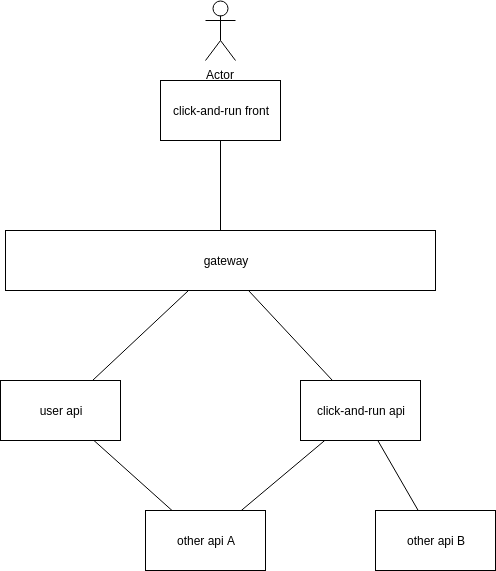
\includegraphics[width=0.7\textwidth]{images/diagrams/gw-archi.png}
    \caption{L'organisation des services et leurs communications (non \gls{a-uml})}
    \label{fig:gw-archi}
\end{figure}

\paragraph{}
Pour comprendre comment c'est possible, il faut d'abord s'intéresser à la manière dont les différents services communiquent entre eux. Comme on peut le voir sur le diagramme \ref{fig:gw-archi}, tous les \glspl{g-server} sont cachés derrière un unique point d'entrée que l'on appelle la passerelle. La passerelle vérifie que les demandes faites aux \glspl{g-server} sont authentifiées. Les demandes faites entre \glspl{g-server} ne sont pas vérifiées car les \glspl{g-server} se font mutuellement confiance.

\begin{figure}[h]
    \centering
    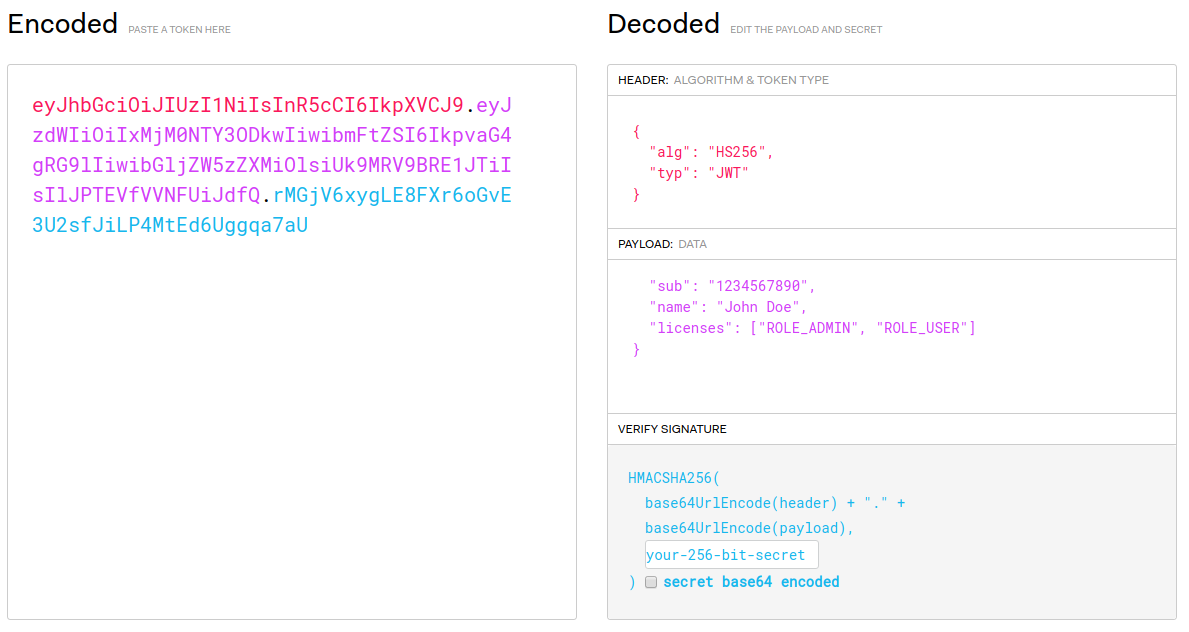
\includegraphics[width=0.7\textwidth]{images/screenshot/jwt-good-secret.png}
    \caption{Un \gls{a-jwt} à gauche et les données décodées à droite}
    \label{fig:jwt-good}
\end{figure}
\begin{figure}[h]
    \centering
    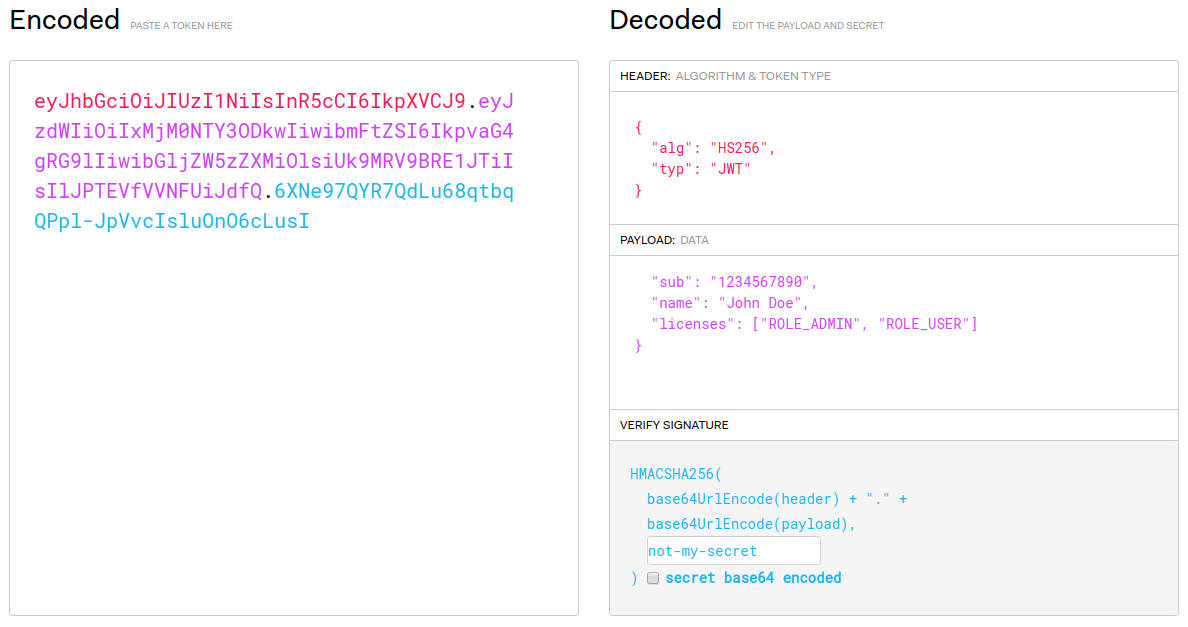
\includegraphics[width=0.7\textwidth]{images/screenshot/jwt-bad-secret.png}
    \caption{Un \gls{a-jwt} avec les mêmes données que sur la figure \ref{fig:jwt-good} mais pas la même signature}
    \label{fig:jwt-bad}
\end{figure}

\paragraph{}
Un \gls{g-client} qui veut s'authentifier fait sa demande à la passerelle.
La passerelle consulte le service des utilisateurs et si l'identifiant et le mot de passe concordent, elle approuve l'authentification.
Elle envoie alors un \gls{a-jwt}, dont on peut observer un exemplaire sur la figure \ref{fig:jwt-good} qui est une sorte de passeport qui déclare l'identité et les droits de l'utilisateur.
Ce \gls{a-jwt} est lisible par tous et est infalsifiable. Son contenu est accompagné d'une signature qui est la résultat de ce même contenu passé par une \gls{g-hash-func}.
La seule manière de reproduire cette signature est disposer de la \gls{g-hash-func} et du secret.
La figure \ref{fig:jwt-bad} illustre ce que l'on obtient sans le bon secret.
Cette formule est présente sur le \gls{a-jwt} et est donc accessible à tous.
Le secret lui n'est connu que par la passerelle et il n'y a donc que elle qui peut produire cette signature.

\paragraph{}
A chaque requête, un client accompagne sa demande de son \gls{a-jwt} et la passerelle reproduit la signature.
Si la signature produite est la même que celle inscrite sur le \gls{a-jwt}, la passerelle transmet la demande, sinon elle la rejette.
Et lorsque les \glspl{g-server} doivent communiquer entre eux pour remplir la demande du client, ils font confiance aux droits indiqués car ils ont été vérifiés par la passerelle.

\paragraph{}
Pour que cela fonctionne, la nouvelle application cliente doit:
\begin{enumerate}
    \item Adresser toutes ses demandes à la passerelle
    \item Implémenter la demande d'authenfication
    \item Fournir le \gls{a-jwt} à chaque requête
\end{enumerate}
Tandis que le nouveau \gls{g-server} doit juste contrôler que les droits d'un utilisateur correspondent au niveau d'autorisation requis pour les ressources qu'il demande.


\subsection{L'internalisation}
\label{subsec:i18n}

\paragraph{}
Chaque valeur textuelle statique\fnmark{} doit être traduite. Seuls des employés d'Altissia auront accès à cette application, il n'est donc pas nécessaire de traduire l'application dans toutes les langues supportées par les autres application d'Altissia\fnmark{}.
\fntext{Toutes données qui ne viennent pas d'une base de données sont dites statiques car elles ne peuvent pas changer pendant la vie de l'application.}
\fntext{Ce qui aurait fait une trentaine de langue dont je n'en connais que trois...}

Il est par contre obligatoire d'être compatible avec le système de localisation qui est déjà mis en place.

Altissia embarque les mécanismes nécessaires à la localisation dans chaque application. Une application peut donc changer de langue sans contacter de \gls{g-server}.

De plus, les informations de localisations sont stockées sur l'application web PhraseApp.
Les localisations devront donc être téléchargées depuis cette dernière.
Le format privilégié pour les applications clientes est le format \gls{a-json}, que l'application devra donc utiliser.

\paragraph{}
L'application cliente devra donc implémenter la localisation seule. C'est le sujet qui est abordé dans la sous section \ref{subsec:i18n-imp}


\subsection{La validation et le traitement des classeurs}
\label{subsec:spreadsheet-use-case}
TODO

\section{Les pages demandées}
\label{subsec:requested-pages}

\paragraph{}
Tous les besoins définis vont se traduire d'une manière ou l'autre en une ou plusieurs pages webs.
Et évidemment, un menu permet de naviguer entre les différentes pages.

\subsection{La page d'accueil}
\label{subsec:home-page}
TODO


\subsection{Les pages du profil}
\label{subsec:profile-page}
TODO


\subsection{Les pages des entités}
\label{subsec:entities-pages}

\paragraph{}
Les pages des entités sont des pages permettant de voir, créer, modifier et supprimer toutes les entrées que peut gérer le site web.
En l'occurrence, les entités sont les apprenants et les licences.

\paragraph{}
Les entités doivent être affichés sont formes de tableaux qui peuvent être triés sur chaque colonne.
Le tri est effectué à partir de la liste complète des entités présentes en base de données et pas uniquement celles qui sont affichées.
Cliquer sur une entité permet d'ouvrir une page qui affiche uniquement les données de celle-ci.

Lorsque l'on clique sur un utilisateur depuis le tableau des licences, on est conduit sur la page de l'utilisateur en question.


\subsection{Les pages de l'administrateur}
\label{subsec:admin-pages}

\paragraph{}
L'\textbf{administrateur} a accès à toute une panoplie d'outils.
Ces pages sont accessibles par un menu qui n'est visible que pour l'\textbf{administrateur}.

Les éléments suivants doivent être présents:
\begin{itemize}
    \item Gateway: Liste les API disponibles
    \item Gestion des utilisateurs: \acrshort{a-crud} sur les listes des \textbf{utilisateurs}
    \item Métriques: Mesures de l'utilisation des ressources de la machine physique sur laquelle est installée l'application
    \item Diagnostics: Liste des services composant l'application et leur état de fonctionnement
    \item Configuration: Liste des propriétés configurables du serveur et leur valeur
    \item Audits: Liste des appels sur les ressources surveillées (ex.: tentative de connexion)
    \item \Glspl{g-log}: Contrôle des niveaux de verbosité des agents de journaux du \gls{g-server}
    \item \gls{a-api}: Liste des ressources exposées par le \gls{g-server} avec exemples d'utilisation
    \item Base de données: Lien vers l'application d'accès à la base de données (ex.: \gls{g-pma})
\end{itemize}

Ces pages doivent correspondre exactement à celles fournies par le générateur de code \Gls{g-jhipster}.
Cet outil est utilisé par Altissia et permet de gagner plusieurs de développements lors de la création de nouveaux projets.
Il génère le code qui constitue le squelette d'un site web et le développeur se l'approprie pour ajouter de nouvelles fonctionnalités par dessus.


\subsection{La page de validation et traitement des classeurs}
\label{subsec:spreadsheet-page}

\paragraph{}
La page de validation et traitement des données est la page centrale de l'application et c'est elle qui va justifier le plus de travail.
Son fonctionnement doit être le plus simple possible.
Un \textbf{utilisateur} doit pouvoir s'en servir sans formation et ses actions ne peuvent pas tromper ses intentions.

\paragraph{}
La page est divisée en trois éléments:
\begin{itemize}
    \item Le récepteur de fichier: il permet de choisir le fichier que l'on valide
    \item Le tableau des résultats: il affiche les résultats de la validation
    \item Le bouton de traitement: il lance le traitement du fichier validé
\end{itemize}

\paragraph{}
Le récepteur de fichier permet de choisir un fichier de deux manières, soit en cliquant dessus, soit en glissant et en déposant un fichier sur lui.
Dans le premier cas, il ouvre le menu système\fnmark{} de l'utilisateur. Dans le second cas, l'utilisateur a cliqué sur le fichier et a maintenu le clic, a glissé le fichier au-dessus du composant et a relâché le clic.
\fntext{Le menu système est le menu prévu par le système d'exploitation installé sur la machine de l'utilisateur}

Dans le cas où le fichier n'est pas compatible, car il n'est pas un fichier Excel ou est corrompu, un message d'erreur renseigne l'utilisateur.
Dans le cas où le fichier est compatible, la validation de son contenu est immédiatement lancée sans autre action de l'utilisateur.

Le nom du fichier sélectionné avec succès est affiché sur le récepteur.

Un doubleclic sur le récepteur vide le fichier.

Des instructions indiquent les actions à prendre en fonction de l'état du fichier: présent ou non présent. % TODO gérer valide et non valide ?

\paragraph{}
Le tableau des résultats affiche les erreurs de validation relevées par le \gls{g-server}.
Le résultat de chaque feuille est affiché dans son propre onglet.
Les erreurs sont divisées en trois tableaux distincts: les problèmes de titre, les erreurs de contenu et les avertissements sur le contenu.
Pour les problèmes de titres, le numéro de colonne, le titre de la colonne, la valeur dans le fichier pour cette colonne et le message d'erreur sont affichés.
Le message d'erreur est exprimé dans un langage intelligible par un \textbf{utilisateur}.
Les mêmes champs sont utilisés par les erreurs et avertissements si ce n'est que la colonne devient une ligne.
Les erreurs sont affichées dans l'ordre des lignes.

\paragraph{}
Le bouton de traitement n'est utilisable que si le fichier a passé la validation.
Son activation envoie le fichier déjà sélectionné et déjà validé pour son traitement.
En cas de succès, ce qui est sensé toujours être le cas, un message de succès apparait et le fichier est vidé du récepteur de fichier.



\section{Le socle d'application de validation et de traitement des classeurs}
\label{sec:spreadsheet-framework}

\paragraph{}
Les outils mis en place doivent au minimum permettre de résoudre les cas d'utilisation proposés.
Mais ils doivent aussi être le plus générique possible afin de pouvoir être appliqués à le plus de cas possibles.
Le socle d'application doit être conçu de manière à ce qu'il soit le plus facile possible d'intégrer de nouveaux outils.

\paragraph{}
Le but de créer un socle d'application plutôt qu'une application concrète est d'être capable de gérer des nouveaux cas avec un temps de développement minimale.
Il est créé libre de droits afin que n'importe qui puisse s'en servir et y contribuer.
Il est donc logique qu'il contienne des outils prêts à l'utilisation, qu'il soit prêt à accueillir des outils inconnus et qu'il soit compatible avec des standards informatiques répandus.

\subsection{Le fonctionnement de Click-and-Run}
\label{subsec:operation}


\subsection{Les outils prêts à l'emploi}
\label{subsec:ready-tools}

\paragraph{}
La plupart des règles de validation ne sont pas propres à un seul classeur, il faut donc les concevoir de façon à ce qu'elles soient utilisables dans d'autres classeurs.

\paragraph{}
Je ne vais donc pas implémenter une règle pour vérifier un format de chaine de caractère précis, mais une règle pour vérifier les formats de manière général.

Je n'ai pas créé une règle qui vérifie qu'un nombre est compris entre 0 et 365, mais deux règles: une pour vérifier qu'une valeur est plus grande qu'une borne et une qui vérifie que la même valeur est inférieure à une autre borne.

Vérifier qu'une valeur fait parti de la liste des services revient à vérifier qu'une valeur est un élément d'un ensemble.

Vérifier que le nom est long de deux à cinquante caractères résulte en une règle qui vérifie la taille d'une chaine de caractères.

Vérifier que l'email est bien défini revient à vérifier qu'il n'est pas \gls{g-null}.


\subsection{Des outils à intégrer}
\label{subsec:host-tools}

\paragraph{}
Certaines règles sont trop spécifiques et il n'est pas possible de les généraliser.
Il est par contre possible de simplifier la vie du développeur qui va devoir les ajouter en prévoyant un système qui va détecter la règle et l'appliquer au bon moment et dans les bons cas.

\paragraph{}
La personne qui veut rajouter une règle dispose de trois points d'entrée:
\begin{itemize}
    \item Le modèle d'une feuille: elle peut associer sa règle au modèle qui représente une ligne
    \item La validation de feuille: elle peut ajouter un service qui sera appelé lors de la validation de la feuille
    \item la validation de classeur: elle peut ajouter un service qui sera appelé lors de la validation du classeur
\end{itemize}
Afin que cela fonctionne, elle doit respecter les formats prévus par mon application.

\paragraph{}
La règle d'un modèle est appliquée sous la forme d'une annotation \textit{javax.validation.constraints}.
C'est un format standard pour la validation que je discute dans la section suivante.

\paragraph{}
Pour la validation d'une feuille ou d'un classeur, le développeur doit créer un service qui doit:
\begin{enumerate}
    \item Indiquer qu'il est capable de traiter le type de données que la validation est en train de vérifier
    \item Implémenter une méthode avec une signature précise qui effectue la vérification
\end{enumerate}
Ce mécanisme correspond au patron de conception de la stratégie.
Il est discuté dans la section \ref{subsec:class-diagram}.


\subsection{Les outils compatibles}
\label{subsec:compatible-tools}


\section{L'architecture mise en place}
\label{sec:architecture}

\paragraph{}
La création d'un site web est une tâche complexe et il convient de mettre en place des outils robustes et éprouvés plutôt que de tout créer de zéro.
Il est aussi primordial de structurer les différents composants de l'application de manière intelligente de manière à obtenir un tout cohérent, maintenable et extensible.
Sachant qu’Altissia gère une quarantaine de services différents, il est impératif que toutes ces applications aient une structure similaire, si ce n'est pas exactement la même.
C'est dans cette optique que j'ai repris bon nombre des technologies employées par mon équipe.

\paragraph{}
Nous utilisons un générateur de code appelé \gls{g-jhipster}.
C'est un projet open source auquel j'ai eu la joie de contribuer au travers d'un module permettant de personnaliser l'\gls{a-orm} générée\cite{noauthor_generator-jhipster-db-helper_nodate}.
Il s'utilise une unique fois au début de chaque projet et il écrit les fondements de la future application.
Je l'ai donc utilisé pour générer l'application de l'interface utilisateur et l'application du \gls{g-server}.

\begin{figure}[ht]
    \centering
    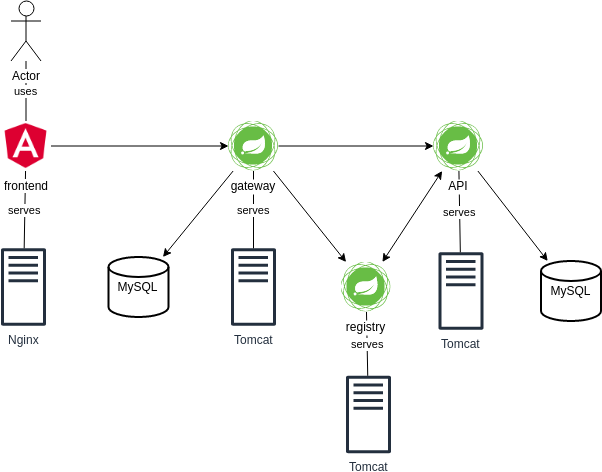
\includegraphics[width=0.7\textwidth]{images/diagrams/gw-archi-detailed.png}
    \caption{Une vue détaillée de l'architecture de l'application Click-and-Run}
    \label{fig:detailed-archi}
\end{figure}

\paragraph{}
La figure \ref{fig:gw-archi} donne un aperçu d'une telle structure.
Voyons avec l'illustration \ref{fig:detailed-archi} sa version détaillée. Je n'y ai inclus que les éléments développés par mes soins et aie omis les éléments externes avec lesquels l'application Click-and-Run interagit.

Détaillons d'abord les noeuds de ce schéma:
\begin{itemize}
    \item \textit{Actor} est l'utilisateur final qui navigue sur nos pages web
    \item Nginx est un \gls{g-server} de fichiers, il sert les fichiers qui lui sont demandés
    \item Tomcat est un serveur applicatif \gls{g-java}, il exécute des applications \gls{g-java} et celles-ci peuvent répondre aux appels qu'on leur fait
    \item \textit{frontend} est l'application Angular qui constitue l'interface que l'utilisateur utilise
    \item \gls{g-mysql} est une base de données
    \item \textit{gateway} est une application \gls{g-spring} qui autorise les demandes et les diriges vers le service demandé
    \item \textit{registry} est une application \gls{g-spring} qui indique où se trouve les services et vérifie leur disponibilité
    \item REST API est une application \gls{g-spring} qui sert des ressources et réponds aux requêtes qu'on lui fait
\end{itemize}
Les flèches indiquent le sens des demandes, le noeud de côté de la queue fait la demande et celui du côté de la pointe répond.
Lorsqu'un verbe est présent sur un lien, le sujet est le noeud situé à l'extrémité du schéma. Tandis que le noeud à l'autre extrémité est le complément d'objet direct.

\paragraph{}
Intéressons-nous d'abord à l'application \gls{g-angular}.
Elle est servie par le \gls{g-server} Nginx.
C'est un \gls{g-server} de fichiers, il n'a pas connaissance leur utilité.
C'est le navigateur internet de l'utilisateur qui interprète les instructions du code contenu dans les fichiers.
Tous les fichiers ne sont pas servis en une seule fois, cela ne serait pas idéal.
Seuls les fichiers nécessaires à afficher la page demandée sont donnés.
Lorsque l'utilisateur navigue dans l'application, cette dernière fera les demandes des fichiers nécessaires à son bon fonctionnement.

\paragraph{}
Peu importe le service que l'application cliente demande, elle doit passer par la passerelle (\textit{gateway} en anglais).

Comme pour chacune des applications \gls{g-java}, un \gls{g-server} Tomcat a la fonction de la faire tourner.
Tomcat est conçu pour exécuter du code \gls{g-java} et écouter les ports réseau de la machine sur laquelle il est installé pour les diriger vers l'application qu'il sert\cite{noauthor_apache_nodate}.

Celle-ci va tout d'abord s'occuper de vérifier la validité du \gls{a-jwt} transmis avec l'appel (l'authentification est traitée en sous-section \ref{subsec:auth-feature}) et ensuite transmettre la demande.
Elle consulte la base de données des utilisateurs pour comparer l'identifiant et le mot de passe lors de l'authentification.
J'ai implémenté un lien direct entre la passerelle et la base de données dans l'application de démonstration, mais dans le cas réel de l'infrastructure logicielle d'Altissia, une passerelle existe déjà et elle s'adresse à un service dédié pour quérir les informations des utilisateurs.
Elle a besoin de travailler de pair avec le registre (\textit{registry} en anglais) pour accomplir son travail.

\paragraph{}
Le registre est une application qui tient à jour un carnet d'adresses des différents services.
Elle se base sur le projet Eureka de Netflix\cite{noauthor_aws_2019} pour gérer la découverte des services.
Lorsqu'un service démarre, il renseigne qu'il est prêt à accomplir son devoir au registre.
Le registre va alors contacter fréquemment tous les services ouverts pour s'assurer de leur disponibilité.

En plus de cette tâche, elle configure les services et prend soin de leur évolutivité.
Un service sera donc configuré selon le registre qui est présent sur l'environnement où il est déployé.
L'évolutivité consiste à adapter les ressources allouées au service en fonction de la charge de travail qu'il endure.
C'est aussi elle qui effectue les mesures présentes dans les pages d'administration (voir sous-section \ref{subsec:admin-pages}).

\paragraph{}
L'\gls{a-api} est le composant qui contient la logique métier.
C'est lui qui s'occupe de la validation et le traitement des classeurs Excel.
Il consulte sa base de données lors de la validation et y insère des données lors du traitement.
Selon l'utilisation qui sera faite de Click-and-Run, cette base de données sera remplacée par des appels à des services externes ou une combinaison des deux.
Altissia a fait le choix de structure ses logiciels en microservices où chaque élément a une responsabilité très précise et il ne fait donc pas sens que Click-and-Run gère des ressources métiers en plus de la logique de validation et traitement pour lequel il a été conçu.

Comme on le voit dans la sous-section \ref{subsubsec:dependency-injection}, la différence entre utiliser un service ou une base de données est minime et passer de l'un à l'autre est trivial.

\paragraph{}
L'interface utilisateur et la passerelle sont développées dans le répertoire de code \href{https://github.com/click-and-run/click-and-run-gw}{click-and-run-gw}\fnmark{} tandis que l'\gls{a-api} et le registre le sont dans le répertoire \href{https://github.com/click-and-run/click-and-run}{click-and-run}\fnmark{}.
\fntext{click-and-run-gw: https://github.com/click-and-run/click-and-run-gw}
\fntext{click-and-run: https://github.com/click-and-run/click-and-run}

\subsection{Le serveur avec Spring}
\label{subsec:server-spring}

\paragraph{}
Le \gls{g-server} est implémenté en utilisant le socle d'application \Gls{g-spring} Boot.
C'est une version de \gls{g-spring} où des choix dogmatiques ont été faits sur la manière dont \gls{g-spring} doit être configuré afin de réduire le travail nécessaire à avoir un \gls{g-server} prêt l'emploi.
\Gls{g-spring} est un projet absolument immense et simplifie la vie du développeur dans nombreux contextes.
Je vais me concentrer ici sur quatre aspects:
\begin{itemize}
    \item La base de données
    \item Le réseau
    \item La sécurité
    \item L'injection de dépendance
\end{itemize}

\subsubsection{La base de données}
\label{subsubsec:spring-data-jpa}

\paragraph{}
Son composant \gls{g-spring} Data \acrshort{a-jpa}, qui est bâti par-dessus le projet \gls{g-hibernate}, gère la connexion a la base de données, la représentation des données sous forme d'objet ainsi que la persistance des données.

Ainsi un développeur n'a plus besoin d'écrire la moindre requête \gls{a-sql}.
Il utilise les fonctions fournies par \gls{g-spring} Data \acrshort{a-jpa}.

On peut par exemple voir ci-dessous la classe qui représente le répertoire dans lequel sont stockées les entités des apprenants:
\begin{lstlisting}[language=Java]
@Repository
public interface LearnerRepository extends JpaRepository<Learner,Long> {
    List<Learner> findAllByLoginIn(Collection<String> loginList);
}
\end{lstlisting}
La méthode \lstinline{findAllByLoginIn} n'est pas prévue de base, mais est construire en utilisant les outils fournis par le \gls{g-framework}.

L'appel \lstinline{learnerRepository.save(learners);} utilise une fonction prévue pour sauvegarder plusieurs apprenants en base de données.
À partir de là, \gls{g-spring} Data \acrshort{a-jpa} s'occupe de créer la requête \gls{a-sql} correspondant.

\subsubsection{Le réseau}
\label{subsubsec:spring-web}

\paragraph{}
Le composant \Gls{g-spring} Web est surement le plus utilisé de \gls{g-spring}.
Il permet de transformer les données reçues par le réseau en objet défini par le code \Gls{g-java}.
En cas de tout écart au scénario nominal, il s'occupe de répondre avec le bon code d'erreur à l'appelant.
Il va par exemple répondre "404 \textit{Not Found}" lorsque la ressource recherchée n'existe pas ou encore "500 \textit{Internal Server Error}" lorsque l'application plante et n'est plus capable de formuler une réponse correcte.

\paragraph{}
Voici par exemple une ressource définie par l'\gls{a-api} de Click-and-Run\fnmark{}:
\fntext{J'ai caché certains détails d'implémentation pour simplifier.}
\begin{lstlisting}[language=Java]
@Timed
@PostMapping(value = "/api/registration/validate", produces = MediaType.APPLICATION_JSON_UTF8_VALUE)
public ResponseEntity<Workbook> validateFile(@RequestParam(name = "file") MultipartFile file) {
    log.debug("REST request to /registration/validate with {}", file.getOriginalFilename());

    Workbook workbook = workbookExtendedService.validateWorkbook(file, new RegistrationWorkbook());

    return ResponseEntity.ok(workbook);
}
\end{lstlisting}
Ce code ne contient que très peu de logique et fait surtout appel aux fonctionnalités de \Gls{g-spring} Web. Il indique à quelle URL la ressource doit répondre, avec quel verbe \gls{a-http}, avec quel paramètre et avec quelle réponse.

\subsubsection{La sécurité}
\label{spring-boot-starter-security}

\paragraph{}
Le composant \gls{g-spring} Security s'occupe de fournir des mécanismes de sécurité pour protéger les différentes ressources du serveur avec un degré de granularité personnalisable.
Il vérifie que chaque demande est légitime.

Pour personnaliser ma configuration du \gls{g-server}, j'ai écrit la fonction suivante dans la classe \lstinline{WebSecurityConfigurerAdapter} qui est utilisée par le \gls{g-framework} pour se configurer.
\begin{lstlisting}[language=Java]
@Override
protected void configure(HttpSecurity http) throws Exception {
    http
        .csrf()
        .disable()
        .headers()
        .frameOptions()
        .disable()
    .and()
        .sessionManagement()
        .sessionCreationPolicy(SessionCreationPolicy.STATELESS)
    .and()
        .authorizeRequests()
        .antMatchers("/api/**").authenticated()
        .antMatchers("/management/health").permitAll()
        .antMatchers("/management/**").hasAuthority(AuthoritiesConstants.ADMIN)
        .antMatchers("/swagger-resources/configuration/ui").permitAll()
    .and()
        .apply(securityConfigurerAdapter());
}
\end{lstlisting}
Cet extrait de code désactive des options qui pourrait débouché sur des vulnérabilités si elles n'étaient pas bien utilisées\cite{noauthor_cross-site_nodate},
active un système de cession sans état\fnmark{}, ce qui est possible grâce à l'utilisation d'une authentification par \gls{a-jwt}
\fntext{Sans état signifie que le \gls{g-server} ne doit pas garder les connections de l'utilisateur en mémoire.}
Et enfin, configure les règles d'accès selon l'URL appelée.

Seuls les utilisateurs authentifiés ont accès aux ressources derrière le chemin \lstinline{/api/**}.
Cela concerne par exemple le chemin \lstinline{/api/registration/validate} utilisé dans l'extrait de code de la sous-section \ref{subsubsec:spring-web}.

Les ressources réservées à l'administrateur sont protégées par le chemin \lstinline{/management/**} à l'exception du chemin \lstinline{/management/health} qui indique si le \gls{g-server} est en bonne santé ou non.

\subsubsection{L'injection de dépendance}
\label{subsubsec:dependency-injection}

\paragraph{}
Dans un programme, une partie d'un logiciel dépend très souvent d'autres parties du logiciel.
Si le bout de code considéré devait lui-même récupérer les bouts de code dont il a besoin, il y serait fortement couplé.
C'est-à-dire qu'il doit connaitre le comportement du code dont il dépend sans quoi il ne sait pas s'en servir.
Ce n'est pas forcément une mauvaise, mais dans certains cas, ce n'est pas idéal.

Un exemple classique est la connexion à la base de données.
Établir la connexion à la base de données requiert des informations comme son emplacement, le nom d'utilisateur et le mot de passe.
Si chaque bout de code qui doit accéder à la base de données devait aussi connaitre ces informations, cela donnerait un code assez complexe.

C'est là qu'intervient l'injection de dépendance.
Plutôt que de devoir instancier\fnmark{} sa dépendance, c'est le \gls{g-framework} qui s'en charge et nous le fournit.
\fntext{Créer un exemplaire concret d'une classe ou d'un modèle}
Dans notre cas, c'est \Gls{g-spring} qui s'en charge.

\paragraph{}
Voici deux applications de l'injection de dépendance:
Voici un premier
\begin{lstlisting}[language=Java]
public LoginUnavailableValidator(LearnerRepository learnerRepository) {
    this.learnerRepository = learnerRepository;
}
// TRUNCATED
learnerRepository.findAllByLoginIn(rowsByLogin.keySet()) // TRUNCATED
\end{lstlisting}
Et un deuxième
\begin{lstlisting}[language=Java]
public ExistingUserValidator(UserExtendedResourceApiClient userExtendedResourceApiClient) {
 this.userExtendedResourceApiClient = userExtendedResourceApiClient;
}
// TRUNCATED
Map<String, UserModel> existingEmail = this.userExtendedResourceApiClient.getUserByLoginMapUsingPOST(emails).getBody();
// TRUNCATED
\end{lstlisting}
Le premier extrait de code fait appel à une base de données tandis que le deuxième appelle un \gls{a-api} en passant par le réseau.
Le développeur ne voit pas la différence, car c'est \Gls{g-spring} qui s'est chargé de fournir les dépendances nécessaires.

En l'occurrence, il peut être intéressant de noter que la méthode du deuxième extrait de code est générée par un outil appelé Swagger sur base du code de la ressource.
Je parle bien d'une ressource telle que celle montrée en exemple dans la sous-section \ref{subsubsec:spring-web}.
Une autre différence est que le premier extrait de code vient de Click-and-Run tandis que le second est un extrait d'un service d'Altissia tournant actuellement en production.
La transition entre les deux est donc triviale.

\paragraph{}
Ce mécanisme est très utile pour implémenter le patron de conception de la stratégie, comme vu dans la sous-section \ref{subsec:class-diagram}.


\subsection{L'interface cliente avec Angular}
\label{subsec:frontend-angular}
TODO




	\chapter{Réalisation}
	\label{ch:implementation}

		TODO

	\chapter{Évolutions immédiates pressenties}
	\label{ch:next-steps}

		TODO

	\chapter{Évaluation du travail}
	\label{ch:auto-critic}

		TODO

	\chapter{Conclusion}
	\label{ch:conclusion}

		TODO
		
	\begin{appendix}
\chapter{Documentation d'un processus d'Altissia launcher}
\label{ch:altissia-launcher-doc}

\paragraph{}
Par soucis de confidentialité, je n'ai finalement pas pu joindre cet extrait de code.

\paragraph{}
Son but était de monter que c'était un processus complexe à suivre et non intuitif.
\chapter{Extrait d'un Excel des questions de test de niveaux}
\label{ch:leveltest-sample}

\paragraph{}
Les questions de tests de niveaux sont des objets complexes que l'on modélise avec plus d'une quarantaine de champs.
J'ai copié un extrait simplifié ci-dessous.

La longueur d'un seul enregistrement était trop long pour tenir sur une feuille, je le présente ici sous forme vertical en rappellant l'entête pour chaque enregistrement.
Dans un soucis de clarté et de lisibilité j'ai activé le retour à la ligne automatique et j'ai remplacé les traits de soulignement avec des espaces pour permettre le retour à la ligne.

\begin{table}[ht]
\begin{tabular}{p{5cm}|p{8cm}}
 & Question 1 \\ \hline
UUID & 2014020611193800100 \\
UUID multipleChoice & 2014020611203209500 \\
MultipleChoice & 1 \\
Open & 0 \\
studyLg & EN \\
locale & EN GB \\
level EU & A2 \\
test name & GRAMMAR \\
online & 1.0 \\
topic tags & (C1 -\textgreater{}) Legal matters \\
grammar tags 1 &  \\
grammar tags 2 &  \\
functions tags &  \\
status & 5-validated \\
type & multiple choice 4 options \\
name & EN 92 \\
instruction multipleChoice four options & Choose the right answer. \\
instruction key & la choose instruction \\
question & - Where are the keys {[}GAP{]} I left on the desk? \\
GAP 1 correct 1 & which \\
GAP 1 incorrect 1 & who \\
GAP 1 incorrect 2 & whom \\
GAP 1 incorrect 3 & those \\
UUID sound & NA \\
sound base reference & NA \\
status sound & NA
\end{tabular}
\end{table}

\begin{table}[ht]
\begin{tabular}{p{5cm}|p{8cm}}
 & Question 2 \\ \hline
UUID & 2014020611232012500 \\
UUID multipleChoice & 2015080312593955700 \\
MultipleChoice & 1 \\
Open & 0 \\
studyLg & EN \\
locale & EN GB \\
level EU & A1 \\
test name & GRAMMAR \\
online & 1.0 \\
topic tags & (A1-\textgreater{}) work and jobs \\
grammar tags 1 & gerund forms \\
grammar tags 2 & passive voice \\
functions tags &  \\
status & 5-validated \\
type & multiple choice 4 options \\
name & EN 94 \\
instruction multiple Choice four options & Choose the right answer. \\
instruction key & la choose instruction \\
question & - I'm going to swim in the sea; do you want to come?- I would love to, but it's impossible for me because I {[}GAP{]} swim! \\
GAP 1 correct 1 & can't \\
GAP 1 incorrect 1 & haven't \\
GAP 1 incorrect 2 & must \\
GAP 1 incorrect 3 & needn't \\
UUID sound & NA \\
sound base reference & NA \\
status sound & NA
\end{tabular}%
\end{table}

\chapter{Extrait du code d'Altissia launcher}
\label{ch:altissia-launcher-code}

\paragraph{}
Par soucis de confidentialité, je n'ai finalement pas pu joindre cet extrait de code.

\paragraph{}
Il avait pour but d'illustrer la complexité de la tâche qu'il fallait relevé.
Ce code était complexe et a été remplacé par un code élégant.

\chapter{La classe \textit{Language.java}}
\label{ch:language-java}

\paragraph{}
Cette classe est une reproduction simplifiée d'une classe utilisée par les services d'Altissia pour manipuler la notion de langue.
L'intérêt est de constater que ce n'est pas une simple liste de langues mais qu'elle définit une nomenclature stricte et classe ses sujets selon les critères d'utilisation.
Toutes langues listée ici est une langue d'interface et certaines sont des langues d'étude.

\paragraph{}
Cela se comprends car il est beaucoup plus difficile de créer le contenu d'apprentissage que traduire les textes des interfaces.
De plus, afficher du contenu de cours dans une langue nécessite d'avoir fait le travail requis pour afficher cette langue.
Il ne reste donc en comparaison aucun effort à faire pour transformer une langue d'étude en une langue d'interface.
Et cet effort est systématiquement fait.

\lstinputlisting[language=java]{pages/appendix/Language.java}
\end{appendix}

	\printbibliography

	\clearpage
\newpage
\pagenumbering{gobble}
\null
\clearpage
 % last page must be empty
\end{document}
